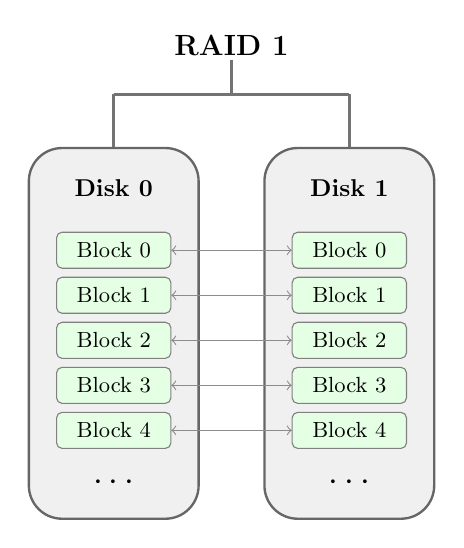
\begin{tikzpicture}[
    x=1cm,y=1cm,
    scale=0.88,
    transform shape,
    every node/.style={font=\small},
    frame/.style={draw=black!60, rounded corners=12pt, line width=0.85pt},
    drive/.style={frame, fill=gray!12, minimum width=2.45cm, minimum height=5.35cm},
    block/.style={draw=black!50, rounded corners=2pt, fill=green!10, minimum width=1.65cm, minimum height=0.52cm},
    bracket/.style={draw=black!55, line width=0.95pt},
    mirror/.style={<->, thin, draw=black!45}
]
    \node[font=\bfseries\large] (title) at (1.7,4.15) {RAID 1};
    \draw[bracket] (0,3.45) -- (3.4,3.45);
    \draw[bracket] (0,2.68) -- (0,3.45);
    \draw[bracket] (3.4,2.68) -- (3.4,3.45);
    \draw[bracket] (1.7,3.45) -- (1.7,3.95);

    \node[drive] (d0) at (0,0) {};
    \node[drive] (d1) at (3.4,0) {};
    \node[font=\bfseries] at (0,2.1) {Disk 0};
    \node[font=\bfseries] at (3.4,2.1) {Disk 1};

    \foreach \y/\lab in {1.20/Block 0,0.55/Block 1,-0.10/Block 2,-0.75/Block 3,-1.40/Block 4} {
        \node[block] at (0,\y) {\lab};
        \node[block] at (3.4,\y) {\lab};
    }

    \foreach \y in {1.20,0.55,-0.10,-0.75,-1.40} {
        \draw[mirror] (0.83,\y) -- (2.57,\y);
    }

    \node[font=\Large] at (0,-2.15) {$\cdots$};
    \node[font=\Large] at (3.4,-2.15) {$\cdots$};
\end{tikzpicture}